
\subsection{板壳单元基本原理}
我们所选用的板壳就是最简单的板壳,对于板选用的是 4 节点 12 自由度矩形 Kirchoff 板,壳在板的基础上加上前面的4Q单元部分. Kirchoff 板遵循平截面假设和直法线假设,因而有

\[
\left\{ \begin{gathered}
u=u_0+z\theta_y \\
v=v_0-z\theta_x \\
w=w_0(x,y)
\end{gathered} \right.
\]

通过假设 $z$ 方向没有剪应变我们可以得到 $\theta_x=\partial x/\partial y, \theta_y=\partial w/\partial x$, 从而

\[
\left\{ \begin{gathered}
\varepsilon_x = -z\frac{\partial^2 w}{\partial x^2} \\
\varepsilon_y = -z\frac{\partial^2 w}{\partial y^2} \\
\gamma_{xy} = -2z\frac{\partial^2 w}{\partial x \partial y}
\end{gathered} \right.
\]

利用上式以及本构关系,只要我们给出了板单元的形函数,我们就能通过积分得到板单元的刚度矩阵.

\subsection{板单元刚度阵的构造}

这里我们采用了彭细荣书中给出的形函数,

\[ \mathbf{N}^T=\left\{
\begin{array}{c}
-\frac{1}{8}(s-1)(t-1)(s^2+s+t^2+t-2)\\ -\frac{1}{8}b(s-1)(t-1)^2(t+1)\\ \frac{1}{8}a(s-1)^2(s+1)(t-1) \\
\frac{1}{8}(s+1)(t-1)(s^2-s+t^2+t-2) \\ \frac{1}{8}b(s+1)(t-1)^2(t+1) \\ \frac{1}{8}a(s+1)^2(s-1)(t-1) \\
-\frac{1}{8}(s+1)(t+1)(s^2-s+t^2-t-2)\\ \frac{1}{8}b(s+1)(t+1)^2(t-1) \\ -\frac{1}{8}a(s+1)^2(s-1)(t+1) \\
\frac{1}{8}(s-1)(t+1)(s^2+s+t^2-t-2) \\ -\frac{1}{8}b(s-1)(t+1)^2(t-1) \\ -\frac{1}{8}a(s-1)^2(s+1)(t+1) \\
\end{array} \right\} \]

根据 $\mathbf{B}=[-\frac{\partial^2}{\partial x^2},-\frac{\partial^2}{\partial y^2},-2\frac{\partial^2}{\partial x \partial y}]^T\mathbf{N}$ 以及 $\mathbf{K}=4ab\mathbf{B}^T\mathbf{D}\mathbf{B}$ 得到总刚度阵.需要说明的是,这里的形函数事实上是一个沿板厚变化的值,但经过积分可以化为弯曲刚度中的一部分.对于得到的刚度阵利用 Zienkiewicz 的原始论文进行初步的验证,二者得到的结果是一致的.

在输出刚度阵时,我们利用 MATLAB 进行完全的积分,并用 char 函数将符号运算输出为字符串,通过少量替换就可以直接在 C++ 中使用.

\subsection{分片验证}

我们在 $[0,1]^2$ 的正方形板构造这样的位移场 $w=x^2-\nu y^2$, 得到一个纯弯场 $M_{11}=-2D(1-\nu^2)$. 利用 $x=0;x=0.3;y=-0.2;y=0$ 四条直线将正方形板分割成九个分片,对应的将法线沿 $x$ 轴方向边界上的 $y$ 向弯矩分配到每个点上.具体输入文件见 plate\_patch\_test, 可见位移基本准确,误差在浮点数范围内.

\subsection{单点位移收敛率分析}

取四边简支的正方形薄板,薄板大小同上,取 $E=230.4GPa,\nu=0.2$, 在中央加一集中载荷 $P$, 根据弹性力学可以得到其级数解 $w=\frac{16P}{D\pi^4}\sum\limits_{m=0}^{\infty}\sum\limits_{n=0}^{\infty} \frac{(-1)^(m+n)}{((2m+1)^2+(2n+1)^2)^2}\sin\frac{m\pi x_1}{2}\sin$ $\frac{n\pi x_2}{2}$, 通过数值方法得到其中央的最大挠度为 $\frac{0.04640335P}{D}=0.232017$. 对于 $2\times 2,4\times 4,8\times 8$ 依次进行求解,得到的结果的对数误差如图\ref{platecvg}:

\begin{figure}[htbp]
  \centering
  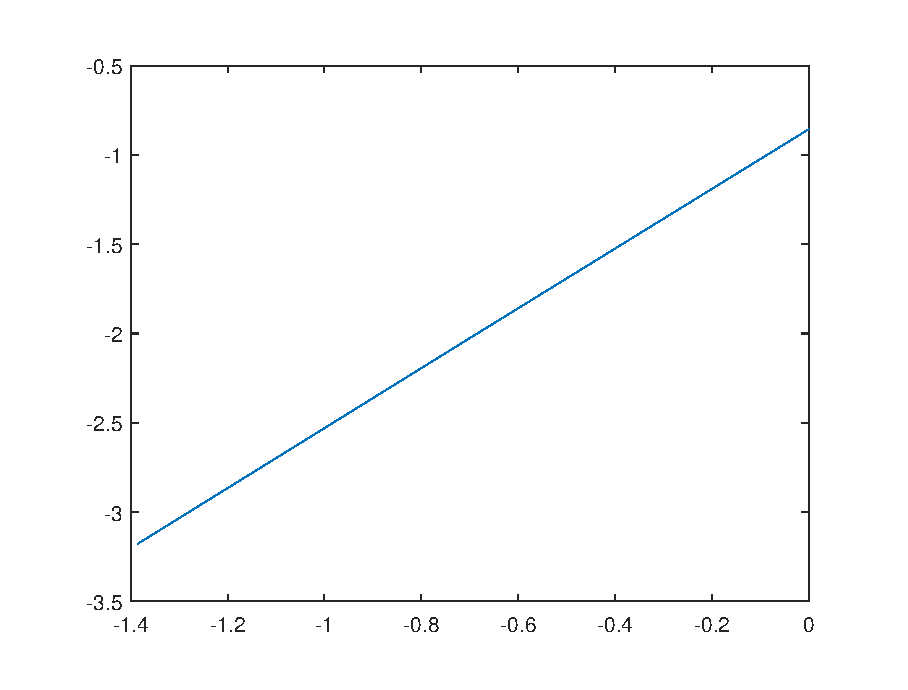
\includegraphics[width=6cm]{plateconvergence}
  \caption{中点收敛率分析}
  \label{platecvg}
\end{figure}
对于板,其形函数是三次以上的,而且构造的位移场是级数场,因而中点不是其高斯点.发现收敛率为 $1.67$ ,考虑到构造的不是多项式场,认为这样的收敛率是可以满意的,也与书上的结果符合,因此认为该板是收敛的.具体文件见 downpress1, downpress2, downpress3.

\subsection{板壳单元自由度的约束}
由于板单元与平板壳单元只能提供面外两个方向的旋转刚度,却不能提供面内的旋转刚度,因此我们需要约束相关方向的自由度,同时放开面外的旋转自由度.因此我们在梁解放相关自由度后还有对于板壳单元自由度的处理:当输入的自由度不含旋转自由度时,对板壳单元所在各点进行判断,如果各点的某一坐标(比如 $z$ 坐标)相差不超过浮机器精度,认为该单元的法向是沿 $z$ 方向的,从而释放对应几个点 $x,y$ 方向的自由度而 $z$ 方向自由度不变,这样也不会影响已经具有刚度而被放开的自由度.

对于倾斜方向的板需要约束变分条件才能解决,目前不在我们程序解决的范围之内.

\subsection{板壳单元输入格式}
板单元和平板壳单元的代号分别为 6 和 7 ,输入材料时传递三个参数,按顺序分别为单元的杨氏模量 $E$, 单元的泊松比 $\nu$ 和单元的厚度 $h$. 每个单元只需要输入四个顶点的单元编号.

